\documentclass[10pt,a4paper]{article}
\usepackage[margin=2.2cm]{geometry}
\usepackage[T1]{fontenc}
\usepackage[utf8]{inputenc}
\usepackage{lmodern}
\usepackage{microtype}
\usepackage{graphicx}
\usepackage{booktabs}
\usepackage{tabularx}
\usepackage{amsmath,amssymb}
\usepackage{xcolor}
\usepackage{enumitem}
\usepackage{caption}
\usepackage{placeins}
\usepackage[colorlinks=true,linkcolor=blue!50!black,urlcolor=blue!50!black]{hyperref}
\captionsetup{font=small,labelfont=bf}
\setlist{nosep,leftmargin=1.3em}

\definecolor{mA}{HTML}{2A78D6}
\definecolor{mB}{HTML}{EB6834}
\definecolor{mC}{HTML}{1BAF7A}
\newcommand{\A}{\textcolor{mA}{\textbf{A}}}
\newcommand{\B}{\textcolor{mB}{\textbf{B}}}
\newcommand{\C}{\textcolor{mC}{\textbf{C}}}
\newcommand{\up}{$\uparrow$}
\newcommand{\dn}{$\downarrow$}

\newcommand{\paramsA}{54.5}
\newcommand{\meanbpbA}{1.778}
\newcommand{\bpbAweb}{1.450}
\newcommand{\bpbAcode}{2.423}
\newcommand{\bpbAmath}{1.921}
\newcommand{\bpbAwiki}{1.320}
\newcommand{\bpbAatest}{1.266}
\newcommand{\hellaswagA}{28.4}
\newcommand{\arceasyA}{31.6}
\newcommand{\piqaA}{52.3}
\newcommand{\lambadaA}{11.1}
\newcommand{\lambadapplA}{710}
\newcommand{\tputA}{142}
\newcommand{\decodeA}{6.6}
\newcommand{\vramA}{0.58}
\newcommand{\tokensA}{0.38}
\newcommand{\flopsA}{1.25\times10^{17}}
\newcommand{\kwhpreA}{0.09}
\newcommand{\kwhtotA}{0.1}
\newcommand{\hoursA}{7.1}
\newcommand{\tppA}{7}
\newcommand{\paramsB}{100.7}
\newcommand{\meanbpbB}{1.052}
\newcommand{\bpbBweb}{1.109}
\newcommand{\bpbBcode}{0.755}
\newcommand{\bpbBmath}{1.219}
\newcommand{\bpbBwiki}{1.123}
\newcommand{\bpbBatest}{1.438}
\newcommand{\hellaswagB}{33.6}
\newcommand{\arceasyB}{47.7}
\newcommand{\piqaB}{61.6}
\newcommand{\lambadaB}{24.5}
\newcommand{\lambadapplB}{22}
\newcommand{\tputB}{66}
\newcommand{\decodeB}{15.0}
\newcommand{\vramB}{0.86}
\newcommand{\tokensB}{3.42}
\newcommand{\flopsB}{2.26\times10^{18}}
\newcommand{\kwhpreB}{7.93}
\newcommand{\kwhtotB}{10.5}
\newcommand{\hoursB}{15.7}
\newcommand{\tppB}{34}
\newcommand{\meanbpblongB}{0.979}
\newcommand{\paramsC}{343.7}
\newcommand{\meanbpbC}{0.991}
\newcommand{\bpbCweb}{1.071}
\newcommand{\bpbCcode}{0.721}
\newcommand{\bpbCmath}{1.096}
\newcommand{\bpbCwiki}{1.075}
\newcommand{\bpbCatest}{1.326}
\newcommand{\hellaswagC}{35.7}
\newcommand{\arceasyC}{56.0}
\newcommand{\piqaC}{66.6}
\newcommand{\lambadaC}{32.9}
\newcommand{\lambadapplC}{11}
\newcommand{\tputC}{27}
\newcommand{\decodeC}{31.2}
\newcommand{\vramC}{2.21}
\newcommand{\tokensC}{5.46}
\newcommand{\flopsC}{1.22\times10^{19}}
\newcommand{\kwhpreC}{51.10}
\newcommand{\kwhtotC}{99.5}
\newcommand{\hoursC}{101.3}
\newcommand{\tppC}{16}
\newcommand{\meanbpblongC}{0.921}
\newcommand{\nonpadA}{39}
\newcommand{\uniqueA}{37}
\newcommand{\benchN}{2000}

\newcommand{\hsgptTwo}{34.8}
\newcommand{\lambgptTwo}{34.5}
\newcommand{\arcgptTwo}{44.5}
\newcommand{\piqagptTwo}{62.2}
\newcommand{\bpbgptTwo}{1.243}
\newcommand{\hsgptTwoMed}{38.6}
\newcommand{\lambgptTwoMed}{44.1}
\newcommand{\arcgptTwoMed}{49.4}
\newcommand{\piqagptTwoMed}{67.3}
\newcommand{\bpbgptTwoMed}{1.107}
\newcommand{\hspythiaS}{33.7}
\newcommand{\lambpythiaS}{34.8}
\newcommand{\arcpythiaS}{44.3}
\newcommand{\piqapythiaS}{61.8}
\newcommand{\bpbpythiaS}{1.024}
\newcommand{\hspythiaM}{38.2}
\newcommand{\lambpythiaM}{51.2}
\newcommand{\arcpythiaM}{52.8}
\newcommand{\piqapythiaM}{68.2}
\newcommand{\bpbpythiaM}{0.885}
\newcommand{\hsoptS}{34.5}
\newcommand{\lamboptS}{39.4}
\newcommand{\arcoptS}{43.2}
\newcommand{\piqaoptS}{61.8}
\newcommand{\bpboptS}{1.194}
\newcommand{\hssmolS}{38.9}
\newcommand{\lambsmolS}{43.8}
\newcommand{\arcsmolS}{64.3}
\newcommand{\piqasmolS}{68.6}
\newcommand{\bpbsmolS}{0.895}
\newcommand{\hssmolM}{43.5}
\newcommand{\lambsmolM}{54.4}
\newcommand{\arcsmolM}{70.3}
\newcommand{\piqasmolM}{72.7}
\newcommand{\bpbsmolM}{0.796}
\newcommand{\flopsratioCgptS}{18}
\newcommand{\tokratioCgptS}{55}


\title{\textbf{How Do Our Models Stack Up?}\\[2pt]
\large Models \A{}, \B{} and \C{} vs.\ GPT-3 and seven open small language models}
\author{Model comparison report --- external baselines}
\date{November 2026}

\begin{document}
\maketitle

\begin{abstract}
\noindent We place three in-house language models in context:
\begin{itemize}
  \item \A{}: \paramsA\,M parameters, GPT-2 style, \tokensA\,B training tokens.
  \item \B{}: \paramsB\,M parameters, Llama style, \tokensB\,B tokens.
  \item \C{}: \paramsC\,M parameters, Llama style, \tokensC\,B tokens.
\end{itemize}
We compare them with the original GPT-3 family (Brown et al., 2020) and with seven openly released small models: GPT-2 124M and 355M, OPT-125M, Pythia-160M and 410M, and SmolLM2-135M and 360M.
GPT-3 numbers are taken from the paper. Every other model, ours included, was run through one identical harness: the same raw text for bits per byte (bpb), the same benchmark items and prompts, and the same GPU.

The main findings:
\begin{itemize}
  \item \textbf{C vs.\ GPT-3 Small.} \C{} matches or beats GPT-3 Small on HellaSwag, ARC-Easy and PIQA, using 1/\flopsratioCgptS{} of its training compute and \tokratioCgptS$\times$ fewer tokens.
  \item \textbf{B and C vs.\ GPT-2.} \B{} and \C{} model text better than the GPT-2 models of matching size, and beat them on ARC-Easy.
  \item \textbf{The modern models lead.} Models trained on far more tokens (Pythia: 300\,B; SmolLM2: 2--4\,T) beat \C{} on almost every metric, and SmolLM2-360M is the strongest model tested. At this scale the training-token budget, not the architecture, separates the models.
  \item \textbf{A trails everything.} \A{} is below every baseline on every metric.
\end{itemize}
\end{abstract}

\section{The contenders}

\begin{table}[h]
\centering\scriptsize
\setlength{\tabcolsep}{3.5pt}
\resizebox{\linewidth}{!}{%
\begin{tabular}{lllrrrrlrl}
\toprule
Model & Year & Family & Layers & $d_\text{model}$ & Heads (KV) & Ctx & Positions / MLP & Vocab & Training data \\
\midrule
GPT-3 Small / Medium$^\dagger$ & 2020 & GPT & 12 / 24 & 768 / 1024 & 12 / 16 & 2048 & learned / GELU & 50k & 300B tok.\ (CC, WebText2, books, Wiki) \\
GPT-2 124M / 355M & 2019 & GPT & 12 / 24 & 768 / 1024 & 12 / 16 & 1024 & learned / GELU & 50\,257 & WebText ($\approx$40\,GB) \\
OPT-125M & 2022 & GPT & 12 & 768 & 12 & 2048 & learned / ReLU & 50\,272 & 180B tok. \\
Pythia-160M / 410M & 2023 & GPT-NeoX & 12 / 24 & 768 / 1024 & 12 / 16 & 2048 & 25\% RoPE, parallel / GELU & 50\,304 & 300B tok.\ (The Pile) \\
SmolLM2-135M & 2024 & Llama & 30 & 576 & 9 (3) & 8192 & RoPE / SwiGLU & 49\,152 & 2T tok. \\
SmolLM2-360M & 2024 & Llama & 32 & 960 & 15 (5) & 8192 & RoPE / SwiGLU & 49\,152 & 4T tok. \\
\midrule
\A{} (ours) & 2026 & GPT & 12 & 512 & 8 & 512 & learned / GELU & 32\,000 & \tokensA B tok.\ (37M unique $\times$10 epochs) \\
\B{} (ours) & 2026 & Llama & 12 & 768 & 12 (4) & 4096 & RoPE / SwiGLU & 32\,768 & \tokensB B tok.\ + mid/post-training \\
\C{} (ours) & 2026 & Llama & 28 & 1024 & 16 (4) & 4096 & RoPE / SwiGLU & 32\,768 & \tokensC B tok.\ + mid/post-training \\
\bottomrule
\end{tabular}}
\caption{Architectures. Open-model values are read from each model's released \texttt{config.json}. $^\dagger$GPT-3 values are from Table~2.1 of the paper, and GPT-3 alternates dense and locally banded sparse attention. Training-token counts are as reported by each model's authors.}
\label{tab:arch}
\end{table}

\noindent Two things to note about the line-up:
\begin{itemize}
  \item \textbf{A and B are closest to the 125M class,} alongside GPT-2 124M, OPT-125M, Pythia-160M, SmolLM2-135M and GPT-3 Small.
  \item \textbf{C belongs to the 350M class,} alongside GPT-2 355M, Pythia-410M, SmolLM2-360M and GPT-3 Medium.
\end{itemize}
The defining difference is the training-token budget, which ranges over four orders of magnitude: from 0.4\,B tokens for A to 4\,T for SmolLM2-360M.

\section{Method}

\begin{itemize}
  \item \textbf{Language-modelling quality: bits per byte (bpb).} Each model scores the same UTF-8 text with its own tokenizer:
    \begin{itemize}
      \item four held-out domains (web, code, math, Wikipedia; about 0.55--0.6\,MB each);
      \item plus A's lower-cased test split (``A-test'').
    \end{itemize}
    Each document starts from BOS and is scored in 512-token windows. bpb is the total negative log-likelihood in bits divided by the original byte count, so it is comparable across tokenizers.
  \item \textbf{Zero-shot benchmarks.} Each answer is scored by its log-likelihood:
    \begin{itemize}
      \item HellaSwag and PIQA use length-normalised accuracy; ARC-Easy uses raw accuracy.
      \item LAMBADA (the OpenAI version) requires an exact greedy prediction of the final word.
      \item The items are the first 2\,000 of each set, and all 1\,838 for PIQA, identical for every measured model.
    \end{itemize}
  \item \textbf{Speed.} We measure fp16 prefill throughput at batch 8 and sequence length 512 on one RTX~2070~Super.
  \item \textbf{GPT-3.} Its numbers are the published zero-shot values from Table~H.1 of Brown et al.\ (2020), checked against the paper. They come from full test sets under the paper's own protocol, and were not re-measured here.
  \item \textbf{Harness check.} Our own checkpoints reproduce their training-log losses and benchmark scores. For example, C scores 35.7\% on HellaSwag here and 35.75\% in its own pipeline log.
\end{itemize}

\section{Results}

\subsection{The full scoreboard}

\begin{table}[h]
\centering\scriptsize
\setlength{\tabcolsep}{4pt}
\begin{tabular}{llrrrrrrrrr}
\toprule
Model & Year & Params & Train tok. & Ctx & HellaSw. & ARC-E & PIQA & LAMB. acc & LAMB. ppl & bpb \\
\midrule
GPT-3 Small$^\dagger$ & 2020 & 125M & 300B & 2048 & 33.7 & 43.6 & 64.6 & 42.7 & 18.6 & -- \\
GPT-3 Medium$^\dagger$ & 2020 & 356M & 300B & 2048 & 43.6 & 46.5 & 70.2 & 54.3 & 9.1 & -- \\
GPT-3 Large$^\dagger$ & 2020 & 760M & 300B & 2048 & 51.0 & 53.0 & 72.9 & 60.4 & 6.5 & -- \\
GPT-3 XL$^\dagger$ & 2020 & 1,320M & 300B & 2048 & 54.7 & 53.8 & 75.1 & 63.6 & 5.4 & -- \\
GPT-3 175B$^\dagger$ & 2020 & 174,600M & 300B & 2048 & 78.9 & 68.8 & 81.0 & 76.2 & 3.0 & -- \\
\midrule
GPT-2 124M & 2019 & 124M & n/r & 1024 & 34.8 & 44.5 & 62.2 & 34.5 & 15.2 & 1.243 \\
GPT-2 355M & 2019 & 355M & n/r & 1024 & 38.6 & 49.4 & 67.3 & 44.1 & 8.9 & 1.107 \\
OPT 125M & 2022 & 125M & 180B & 2048 & 34.5 & 43.2 & 61.8 & 39.4 & 10.9 & 1.194 \\
Pythia 160M & 2023 & 162M & 300B & 2048 & 33.7 & 44.3 & 61.8 & 34.8 & 12.8 & 1.024 \\
Pythia 410M & 2023 & 405M & 300B & 2048 & 38.2 & 52.8 & 68.2 & 51.2 & 5.5 & 0.885 \\
SmolLM2 135M & 2024 & 135M & 2T & 2048 & 38.9 & 64.3 & 68.6 & 43.8 & 7.8 & 0.895 \\
SmolLM2 360M & 2024 & 362M & 4T & 2048 & 43.5 & 70.3 & 72.7 & 54.4 & 5.0 & 0.796 \\
\midrule
\textbf{\A{}} (this work) & 2026 & 54M & 0.38B & 512 & 28.4 & 31.6 & 52.3 & 11.1 & 709.8 & 1.778 \\
\textbf{\B{}} (this work) & 2026 & 101M & 3B & 4096 & 33.6 & 47.7 & 61.6 & 24.5 & 22.5 & 1.052 \\
\textbf{\C{}} (this work) & 2026 & 344M & 5B & 4096 & 35.7 & 56.0 & 66.6 & 32.9 & 10.6 & 0.991 \\
\bottomrule
\end{tabular}

\caption{Zero-shot results. All values are accuracy in percent, except LAMBADA perplexity and bpb (both lower is better). $^\dagger$GPT-3 rows are published values. Every other row was measured here on identical items. ``Train tok.'' is the pre-training token count reported by the authors (n/r = not reported).}
\label{tab:main}
\end{table}

\begin{figure}[h]
\centering
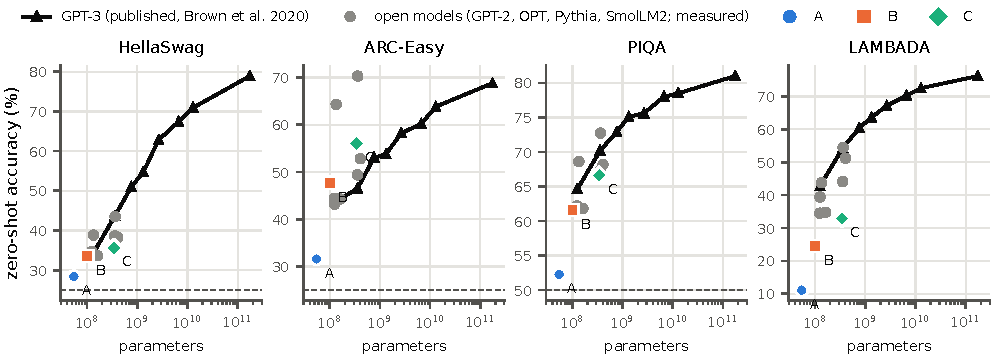
\includegraphics[width=\linewidth]{figs/base_bench_vs_size.pdf}
\caption{Accuracy vs.\ parameter count. The black line is the published GPT-3 family. Grey points are the open models, measured here. Coloured markers are our models. Dashed lines mark chance.}
\label{fig:size}
\end{figure}

The GPT-3 curve in Figure~\ref{fig:size} is a useful yardstick: it shows what 300\,B tokens buy at each model size.
\begin{itemize}
  \item \textbf{On ARC-Easy,} \C{} and \B{} sit \emph{above} the GPT-3 curve, and both SmolLM2 models sit far above it. This reflects the educational, science, code and math content of modern data mixes.
  \item \textbf{On HellaSwag and PIQA,} \C{} lands near GPT-3 Small, a model about a third of its size.
  \item \textbf{On LAMBADA,} all three of our models are well below the curve.
\end{itemize}

\subsection{Head-to-head: C against the 350M class and GPT-3}

\begin{table}[h]
\centering\small
\begin{tabular}{lrrrrrr}
\toprule
 & HellaSwag & ARC-Easy & PIQA & LAMBADA & bpb \dn & Train tokens \\
\midrule
GPT-3 Small (125M)$^\dagger$ & 33.7 & 43.6 & 64.6 & 42.7 & -- & 300B \\
GPT-3 Medium (350M)$^\dagger$ & 43.6 & 46.5 & 70.2 & 54.3 & -- & 300B \\
GPT-2 355M & \hsgptTwoMed & \arcgptTwoMed & \piqagptTwoMed & \lambgptTwoMed & \bpbgptTwoMed & n/r \\
Pythia-410M & \hspythiaM & \arcpythiaM & \piqapythiaM & \lambpythiaM & \bpbpythiaM & 300B \\
SmolLM2-360M & \textbf{\hssmolM} & \textbf{\arcsmolM} & \textbf{\piqasmolM} & \textbf{\lambsmolM} & \textbf{\bpbsmolM} & 4T \\
\midrule
\C{} (ours) & \hellaswagC & \arceasyC & \piqaC & \lambadaC & \meanbpbC & \tokensC B \\
\bottomrule
\end{tabular}
\caption{C against models of the same size, plus GPT-3 Small. $^\dagger$GPT-3 values are published.}
\label{tab:h2h}
\end{table}

\noindent What Table~\ref{tab:h2h} shows for \C{}:
\begin{itemize}
  \item \textbf{Ahead of GPT-2 355M,} the closest model of the same size and era-defining architecture, on bpb (\meanbpbC{} vs.\ \bpbgptTwoMed) and on ARC-Easy.
  \item \textbf{Behind GPT-2 355M} on HellaSwag, PIQA and especially LAMBADA.
  \item \textbf{Behind Pythia-410M and SmolLM2-360M} on every metric except Pythia's ARC-Easy. Those models saw 55$\times$ and 730$\times$ more tokens.
\end{itemize}

\subsection{Language-modelling quality across domains}

\begin{figure}[h]
\centering
\begin{minipage}{0.4\linewidth}\centering
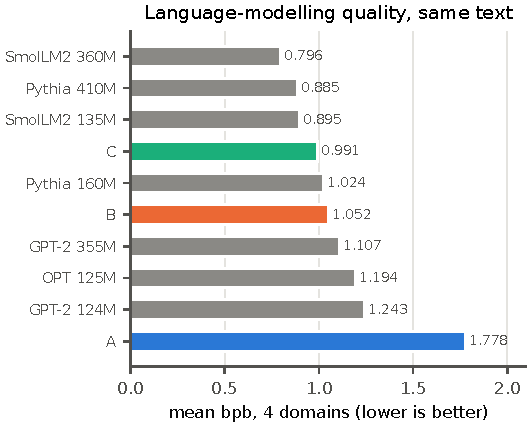
\includegraphics[width=\linewidth]{figs/base_bpb_rank.pdf}
\end{minipage}\hfill
\begin{minipage}{0.58\linewidth}\centering
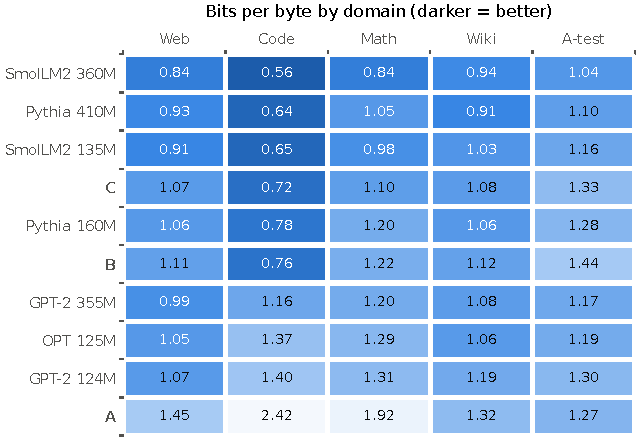
\includegraphics[width=\linewidth]{figs/base_domain_heatmap.pdf}
\end{minipage}
\caption{Left: mean bpb over the four domains, ranked. Right: bpb per domain, with rows sorted by the mean. Bold rows are our models.}
\label{fig:bpb}
\end{figure}

Figure~\ref{fig:bpb} shows how the models rank on raw text:
\begin{itemize}
  \item \textbf{Overall,} \C{} ranks 4th of 10 and \B{} 6th, ahead of all three 2019--2022 models (GPT-2 124M and 355M, OPT-125M).
  \item \textbf{On code,} our models are much stronger than GPT-2 and OPT, whose training data contained almost no source code.
  \item \textbf{On Wikipedia and A-test,} Pythia and GPT-2 355M do relatively well, because their corpora contain more encyclopedic and news text.
  \item \textbf{A} is last on every domain except its own A-test, where it beats B, C, GPT-2 124M and (narrowly) Pythia-160M.
\end{itemize}

\subsection{Data and compute efficiency}

\begin{figure}[h]
\centering
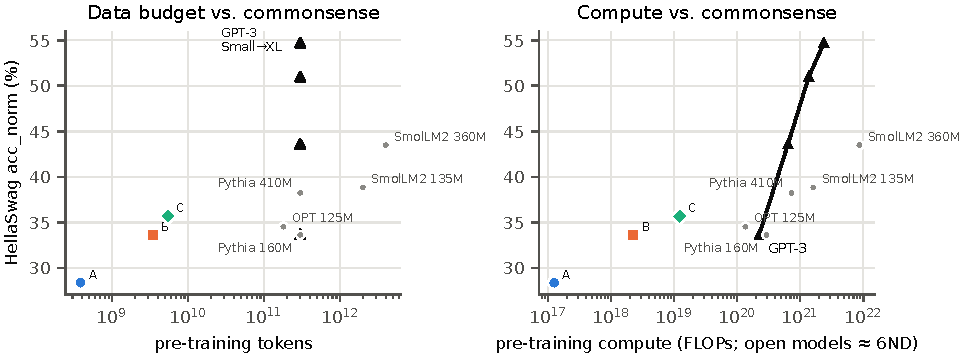
\includegraphics[width=\linewidth]{figs/base_efficiency.pdf}
\caption{HellaSwag vs.\ pre-training tokens (left) and vs.\ pre-training compute (right). Compute for open models is estimated as $6ND$; GPT-3 compute is from Table~D.1 of the paper. GPT-2 is omitted because its token count was not published.}
\label{fig:eff}
\end{figure}

Figure~\ref{fig:eff} shows how efficiently each model turns data and compute into accuracy:
\begin{itemize}
  \item \textbf{Per token of data,} B and C are by far the most efficient models in the comparison: they reach 33--36\% HellaSwag with 3--5\,B tokens, while the baselines needed 180\,B--4\,T tokens to reach about 34--44\%.
  \item \textbf{Per FLOP,} C reaches GPT-3 Small's HellaSwag score with about 5\% of its compute.
  \item \textbf{The gain is not free.} Accuracy keeps rising with tokens, so the extra data of the modern models still buys a large margin.
\end{itemize}

\subsection{Speed vs.\ quality}

\begin{figure}[h]
\centering
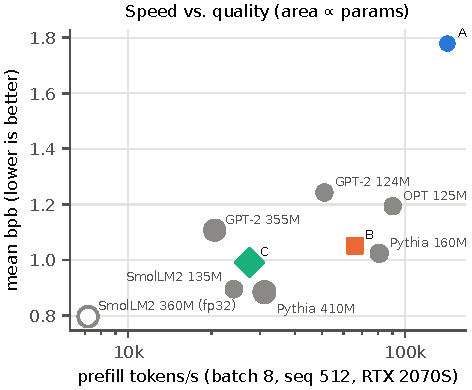
\includegraphics[width=0.55\linewidth]{figs/base_speed_quality.pdf}
\caption{Prefill throughput vs.\ mean bpb on one RTX~2070~Super (fp16, batch 8, sequence length 512). Marker area is proportional to parameters. SmolLM2-360M (hollow marker) had to run in fp32 because its activations overflow fp16, so its speed is not comparable.}
\label{fig:speed}
\end{figure}

On speed vs.\ quality (Figure~\ref{fig:speed}):
\begin{itemize}
  \item \textbf{B} sits just behind Pythia-160M, which is both slightly faster and slightly better in bpb.
  \item \textbf{SmolLM2-135M} is deep and narrow (30 layers, $d{=}576$), so it is slow for its size.
  \item \textbf{C} is about as fast as Pythia-410M and SmolLM2-135M.
  \item \textbf{A} is the fastest model, but far behind on quality.
\end{itemize}

\section{Verdict per model}

\begin{description}[leftmargin=1.2em]
\item[\A{} (54M).] Below every baseline on every metric. It is data-starved: about 7 tokens per parameter, repeated over 10 epochs. It also lower-cases its input and is limited to 512 tokens. Its closest peers, GPT-2 124M and OPT-125M, are 2--3 years older designs, yet clearly better because they saw 100--500$\times$ more data. Value: an educational baseline.
\item[\B{} (101M).] Comparable to GPT-2 124M and OPT-125M on commonsense (HellaSwag \hellaswagB{} vs.\ \hsgptTwo/\hsoptS). Better on ARC-Easy and bpb, and weaker on LAMBADA. Unlike any of the baselines, it is instruction-tuned and chat-capable.
\item[\C{} (344M).] Roughly the level of GPT-3 Small, and of GPT-2 355M on bpb and ARC-Easy. It is the most data-efficient model in the comparison. With B, it is one of only two instruction-tuned, chat-capable models here, and with B and SmolLM2, one of the few with a context window of at least 4k tokens. It is clearly behind the 2023--24 models trained on 300\,B--4\,T tokens, with LAMBADA as its weakest point.
\end{description}

\paragraph{Recommendation.}
For C, the cheapest path to a better model is more pre-training tokens, not a larger network. Pythia-410M, a similar size trained on 55$\times$ more tokens, gains about 18 LAMBADA points and 0.1\,bpb over C. C's own LAMBADA score was still rising steeply when pre-training stopped.

\section{Caveats}
\begin{itemize}
  \item \textbf{GPT-3 protocol.} GPT-3 numbers come from the paper's protocol (full test sets; ARC uses unconditional-probability normalisation), so they are not strictly comparable with the measured rows. Our 2\,000-item subsets carry about $\pm2$ points of sampling noise.
  \item \textbf{Test-text distribution.} The bpb text comes from the data sources of the B/C pipeline. This favours models trained on similar web, code and math mixes (B, C, SmolLM2), and penalises GPT-2, OPT and Pythia on code.
  \item \textbf{Base vs.\ chat models.} The baselines are base models, while B and C are post-trained chat models scored here without a chat template. Post-training changed C's benchmark scores by under 2 points, but it does slightly raise bpb.
  \item \textbf{Speed.} Speed is measured on consumer hardware without fused kernels. Relative order matters more than absolute numbers.
\end{itemize}

\section*{Reproducing}
\begin{verbatim}
python3 eval_compare.py --model <A|B|C|gpt2|gpt2-medium|opt-125m|pythia-160m|
                                 pythia-410m|smollm2-135m|smollm2-360m> --gpu 0
python3 make_figs.py && python3 make_figs_baselines.py
latexmk -pdf report_baselines.tex
\end{verbatim}
\noindent\textbf{Reference.} T.~Brown et al., \emph{Language Models are Few-Shot Learners}, NeurIPS 2020, arXiv:2005.14165 (Tables 2.1, D.1, H.1).
\end{document}
